\documentclass[12pt]{article}

\usepackage{sbc-template}

\usepackage{url}
\usepackage[brazil]{babel}   
\usepackage[utf8]{inputenc}
\usepackage{amstext}
\usepackage{amsmath}
\usepackage{graphicx}
\usepackage{subfigure}
\usepackage{url}
\usepackage{cite}

\sloppy

\title{Um Estudo sobre a Evolução Temporal de Comunidades Científicas}

\author{Bruno Leite Alves\inst{1} \\ Orientador: Alberto H. F. Laender\inst{1},  
	  Coorientador: Fabrício Benevenuto\inst{1} }
\address{Departamento de Ciência da Computação -- Universidade Federal 
              de Minas Gerais\\
              Belo Horizonte -- MG -- Brazil
  \email{\{bruno.leite,fabricio,laender\}@dcc.ufmg.br}
}

\begin{document} 

\maketitle

\begin{abstract}
In this work, we investigate the role that members of the core of scientific 
communities play in the formation and evolution of their collaboration 
networks. For this, we define a community core based on a metric 
called CoScore, which is an h-index derived metric that captures both, 
the prolificness and the involvement of researchers 
in a community. Our results provide important observations related to community 
formation and evolving patterns. We note, for example, 
that variations on the members of the community core tend to be 
strongly correlated with variations on the network properties.
\end{abstract} 

\begin{resumo} 
Neste trabalho, investigamos o papel que os membros do núcleo de
comunidades científicas têm na formação e evolução de sua redes de
colaboração. Para isso, definimos o núcleo de uma comunidade a partir de
uma métrica denominada CoScore, derivada do índice~h, e que captura tanto
a prolificidade quanto o envolvimento dos pesquisadores na comunidade.
Nossos resultados subsidiam observações importantes relacionadas à
formação e aos padrões de evolução das comunidades. Notamos, por exemplo,
que variações no conjunto de membros que compõem o núcleo das comunidades
tendem a ser fortemente correlacionadas com variações nas propriedades da
própria rede.
\end{resumo}


\section{Introdução}

Desde os seus primórdios, a sociedade tem se organizado em comunidades, ou seja, grupos de indivíduos 
com interesses em comum\footnote{http://www.merriam-webster.com/dictionary/community}. Particularmente, 
a proliferação de novas tecnologias de comunicação baseadas na Internet tem facilitado a rápida 
formação e crescimento de comunidades \textit{online}~\cite{Kleinberg2008}. Comunidades possuem uma grande 
quantidade de características e servem a vários propósitos. Elas podem ser desde pequenos 
grupos hermeticamente comprometidos com temas específicos, como comunidades científicas de determinadas áreas, 
até mesmo grupos de milhões de usuários ligados por um interesse em comum, tais como comunidades 
relacionadas a esporte ou de fãs de uma celebridade.

Geralmente, indivíduos que são socialmente conectados em comunidades tendem a compartilhar interesses comuns
e possuir outras semelhanças. Embora existam muitos fatores que possam determinar a formação de uma comunidade
e o seu crescimento, existem duas forças que explicam a formação de comunidades: influência 
e homofilia~\cite{Cha2010}. Estudos recentes 
têm mostrado evidências que ambas as forças
dependem da identificação de um grupo influente 
de indivíduos com o poder de afetar não somente a estrutura topológica de uma comunidade, 
mas também interferir na difusão e no fluxo de informação da comunidade.

Neste trabalho, apresentamos uma perspectiva diferente e um estudo complementar desse problema. 
Aqui, nos concentramos em estudar os papéis que indivíduos influentes em comunidades científicas
desempenham na evolução das propriedades de tais comunidades. Para esse 
estudo, coletamos dados da biblioteca digital DBLP\footnote{http://dblp.uni-trier.de/} abrangendo 
o período 1964-2012 e envolvendo um total de 43840 publicações e 63601 autores.
A partir desses dados, construímos comunidades científicas, representadas pelas principais conferências
dos SIGs (\textit{Special Interest Groups}) da ACM\footnote{http://www.acm.org/sigs}
(\textit{Association for Computing Machinery}). Então, propomos uma estratégia para definir o 
núcleo de uma dada comunidade científica, juntamente com seus líderes em um dado período de 
tempo. Finalmente, investigamos como os aspectos do núcleo impactam a estrutura topológica da comunidade.

O estudo do núcleo de comunidades científicas pode ser visto de duas perspectivas diferentes: 
sociológica e tecnológica. A 
primeira corresponde à necessidade de entender como partes da sociedade evoluem, enquanto a segunda compreende 
aspectos críticos para muitas aplicações, como predição de links. Tal estudo, entretanto, 
tem sido difícil devido à caracterização de alguns conceitos, como conexões humanas e uma definição apropriada 
de liderança, sendo difícil até mesmo de se reproduzir em grande escala dentro de um laboratório de pesquisa.

A seguir listamos as principais contribuições deste trabalho~\cite{Alves2013}:

\begin{itemize}
 \item Definição de uma métrica, chamada \textit{CoScore}, que captura tanto a prolificidade quanto o 
       envolvimento de um pesquisador em uma comunidade científica;
 \item Definição do conceito de núcleo de uma comunidade a partir da métrica 
 proposta;
 \item Caracterização de mais de vinte comunidades científicas e uma discussão de como a métrica \textit{CoScore} afeta 
       as propriedades topológicas das redes ao longo do tempo;
 \item Visualização das comunidades estudadas\footnote{http://hidra.lbd.dcc.ufmg.br/graphs/}, em que é possível observar os componentes da rede e como os membros 
       dos núcleos se organizam nestes componentes.
 
\end{itemize}

\section{Comunidades}

Dada uma rede social, uma comunidade pode ser compreendida como um grupo denso de nodos dessa rede que possuem mais arestas 
interligando-os entre si, do que arestas interligando-os ao restante da rede. Existem múltiplas definições e estratégias 
para identificar comunidades e elas variam de acordo com o contexto~\cite{Kleinberg2008,Leskovec2010}. No nosso contexto, 
uma comunidade científica pode ser definida em termos de uma grande e consolidada conferência científica capaz de reunir 
pesquisadores que trabalham em uma mesma área de pesquisa ao longo de vários anos.

A fim de construir um conjunto de comunidades científicas, coletamos dados da biblioteca digital DBLP\footnote{http://dblp.uni-trier.de/}.
Para o propósito do nosso 
trabalho, consideramos uma comunidade científica como um grafo em que os nodos 
representam pesquisadores e as arestas ligam os coautores de artigos de uma mesma comunidade. A fim de definir tais 
comunidades, focamos nas publicações das principais conferências (\textit{flagships}) dos SIGs 
da ACM. No total, 22 comunidades científicas de diferentes áreas foram construídas e analisadas.

\section{Definição do Núcleo das Comunidades}

Tentativas anteriores para identificar o núcleo de comunidades científicas são baseadas em abordagens 
algorítmicas que visam identificar conjuntos densos de nodos na rede~\cite{Seifi2012}. Entretanto, 
como planejamos investigar o papel do núcleo na estrutura da rede, qualquer abordagem que faz uso da 
estrutura da rede para identificar tais nodos poderia nos levar a um conjunto de pesquisadores 
enviesado. Em vez disso, focamos no desenvolvimento de uma métrica que quantificasse o envolvimento 
de um pesquisador em uma comunidade científica durante um certo período de tempo. Intuitivamente, 
essa métrica deveria ser capaz de capturar:  (i) a prolificidade de um pesquisador em diferentes 
comunidades usando-se o índice~h, uma métrica largamente adotada para esse propósito, e 
(ii) a frequência do envolvimento daquele pesquisador com a comunidade em um certo 
período de tempo, capturada multiplicando-se o seu índice~h 
ao final desse período pelo número total de publicações desse pesquisador nessa comunidade 
no mesmo período.

Denominamos essa métrica de \textit{Community Score} (\textit{CoScore}) \cite{Alves2013}. 
Mais formalmente, o \textit{CoScore} de um pesquisador $p$ em uma 
comunidade $c$ durante um período de tempo $t$, $\textit{CoScore}_{p,c,t}$, é dado 
pelo seu índice~h ($h_{p,t}$) ao final do período $t$ multiplicado pelo 
número total de suas publicações na comunidade $c$ durante o período $t$ ($\textrm{\#}\text{publicações}_{p,c,t}$),
como expresso pela equação $\textit{CoScore}_{p,c,t} = h_{p,t} \times 
\textrm{\#}\text{publicações}_{p,c,t}$.

Assim, a partir dessa métrica, podemos definir o núcleo de uma comunidade
em um certo período de tempo como sendo formado pelos pesquisadores com os
maiores valores do CoScore. Para isso utilizamos a métrica 
\textit{resemblance}, conforme definida em~\cite{Viswanath2009}, e o
coeficiente angular para determinar dois limiares importantes: o tamanho
do núcleo da comunidade e o tamanho da janela temporal. Esses dois
limiares foram definidos experimentalmente como sendo 10\% da comunidade e
3 anos~\cite{Alves2013}.

\section{Análise da Evolução das Comunidades}

A fim de analisar a evolução das principais propriedades estruturais das comunidades científicas, examinamos várias métricas 
de redes para cada uma das comunidades consideradas. Apresentamos aqui apenas a análise do maior componente fracamente conectado 
(CFC). A análise das demais métricas (assortatividade, caminho 
mínimo médio, coeficiente de agrupamento e grau médio dos nodos) pode ser encontrada na dissertação. 
A Figura~\ref{fig:metrics_largest_connected_component}
mostra como a métrica varia ao longo do tempo. Apresentamos essa métrica para um conjunto de seis 
comunidades científicas selecionadas entre aquelas que mais se estendem ao longo do tempo em nosso conjunto de dados.
Nossas análises são realizadas sob duas perspectivas. A primeira consiste em analisar a evolução da rede ano a ano, acumulando 
nodos e arestas da instância final do grafo. A segunda consiste em analisar instâncias construídas com base em nodos e 
arestas criados em uma janela de tempo predefinida.

\begin{figure}[!htb]
  \vspace{-1.5cm}
  \begin{center}
  \subfigure[Maior CFC final]{%
    \label{fig:largest_connected_component_1_in_1}
    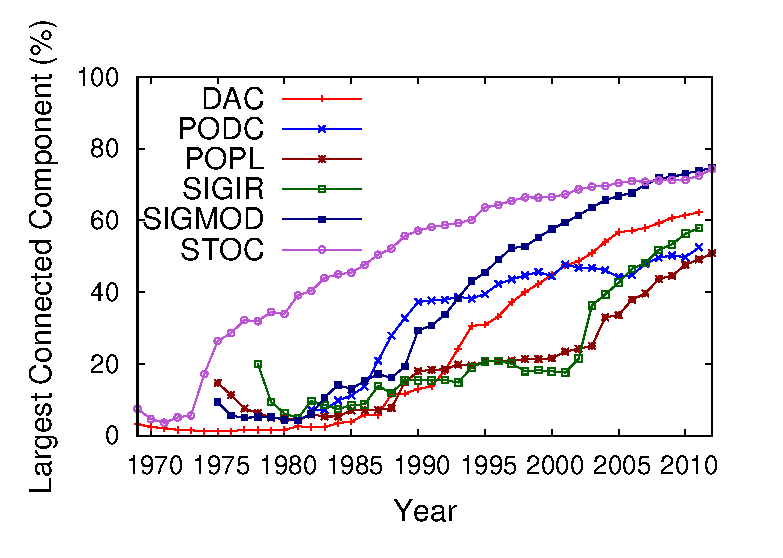
\includegraphics[scale=.5]{../graficos/sigs_metricas_acumuladas_1_em_1_ano/pt_BR/porcentagem_maior_componente_grupo_temporal_web.eps}
  }%
  \subfigure[Maior CFC por janela]{%
    \label{fig:largest_connected_component_slide_window}
    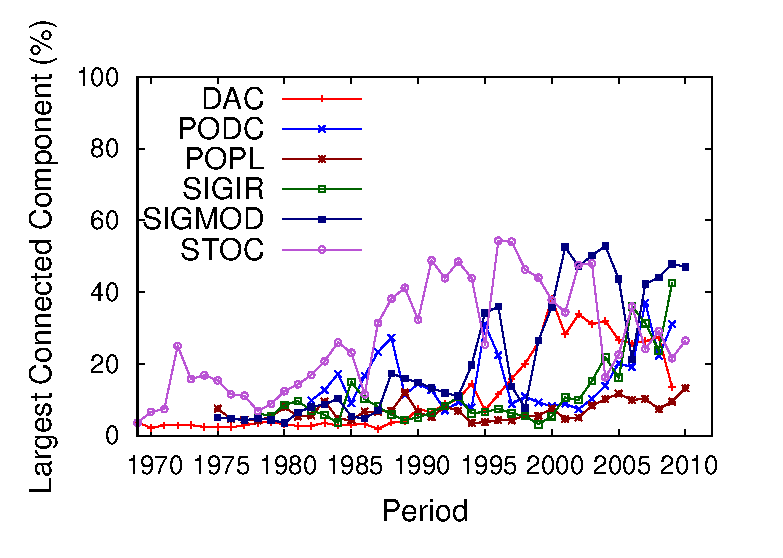
\includegraphics[scale=.5]{../graficos/core_over_time/metricas_tradicionais/pt_BR/porcentagem_maior_componente_slide_window_grupo_temporal_web.eps}
  }%
  \end{center}
  \caption{Maior CFC das comunidades científicas}
  \label{fig:metrics_largest_connected_component}
  \vspace{-0.2cm}
\end{figure}

Notamos a partir da Figura~\ref{fig:metrics_largest_connected_component} que o maior CFC tende a aumentar largamente em função do 
tempo. Isto sugere que na fase inicial as comunidades científicas são formadas por vários grupos de pesquisa pequenos 
e segregados. De forma geral, observamos que as comunidades científicas têm características de evolução semelhantes e que essas 
propriedades são dinâmicas, mudando ao longo do tempo. Mais importante ainda, nossas observações sugerem que 
um pequeno grupo de pesquisadores que fazem parte do núcleo são responsáveis por criar caminhos entre grupos de 
pesquisa menores e mais conectados. A fim de investigar melhor os pesquisadores que fazem parte do núcleo, 
a seguir comparamos membros e não membros dos núcleos das comunidades, bem como o impacto dos membros dos núcleos na estrutura
topológica das comunidades.

\vspace{-0.6cm}
\noindent
\paragraph{Caracterização dos Núcleos das Comunidades.}
\textit{Até que ponto as propriedades dos membros do núcleo diferem dos demais membros das comunidades?} Para responder a essa 
pergunta, calculamos as propriedades de rede para os membros e não membros dos núcleos das comunidades. Consideramos 
a análise de janelas de tempo para compreender as variações que essas duas classes podem ter na medida global. 
A Figura~\ref{fig:metrics_comparing_core_community} mostra o grau médio e o coeficiente de agrupamento médio calculados para 
membros e não membros do núcleo da comunidade SIGMOD. Além disso, 
também medimos a fração de membros do núcleo, bem como dos não membros que estão no maior CFC e calculamos 
o \textit{betweenness} médio de cada um desses grupos de membros.
Como podemos ver, o grau médio dos membros dos núcleos é maior em 
comparação com o dos não membros, que tendem a estabelecer mais conexões em função do tempo.
No entanto, o coeficiente de agrupamento dos membros do núcleo tende a ser 
menor quando comparados com o dos não membros, indicando que eles podem atuar como \textit{hubs}, conectando 
diferentes grupos. Notamos que a fração de membros do núcleo que fazem parte do maior 
CFC, é maior do que a fração de não membros, sugerindo que eles podem estar conectando componentes 
menores. Podemos notar que o \textit{betweenness} médio do núcleo da comunidade é muito maior, 
o que confirma nossas observações.

\begin{figure}[!htb]
  \vspace{-1.4cm}
  \begin{center}
  \subfigure[Coeficiente de agrupamento]{%
    \label{fig:core_com_sigmod_clustering_coefficient}
    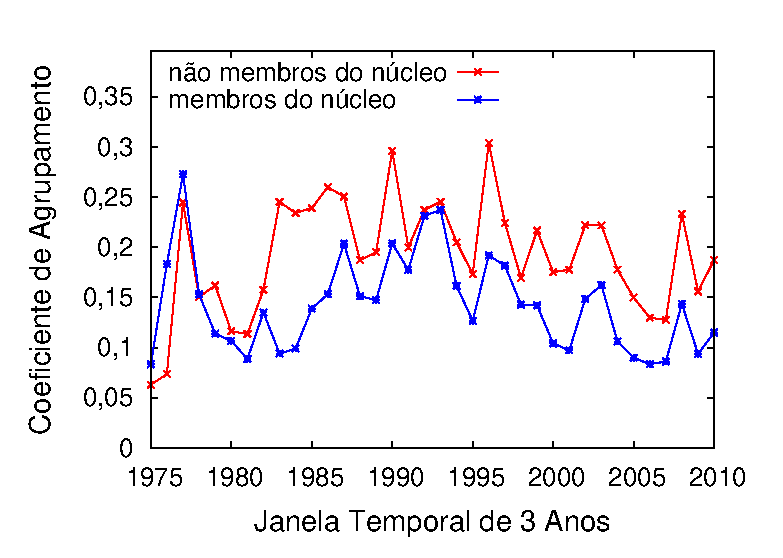
\includegraphics[scale=.45]{../graficos/core_over_time/core_community/pt_BR/sigmod_janela_3_core_coeficiente_agrupamento.eps}
  }
  \subfigure[Grau médio]{%
    \label{fig:core_com_sigmod_average_degree}
    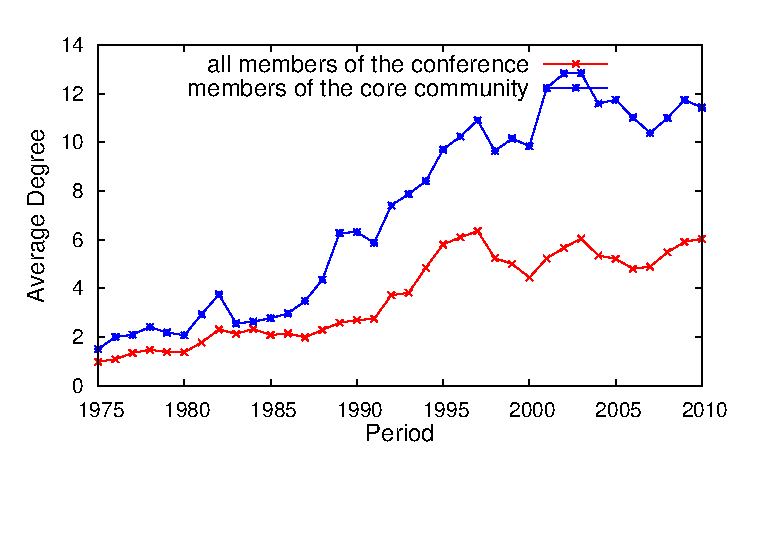
\includegraphics[scale=.45]{../graficos/core_over_time/core_community/pt_BR/sigmod_janela_3_core_grau_medio_nodos.eps}
  }
  
  \subfigure[Maior CFC]{%
    \label{fig:core_com_sigmod_largest_connected_component}
    \includegraphics[scale=.45]{../graficos/core_over_time/core_community/pt_BR/sigmod_janela_3_core_maior_componente_conectado.eps}
  }
  \subfigure[\textit{Betweenness} médio]{%
    \label{fig:core_com_sigmod_betweenness}
    \includegraphics[scale=.45]{../graficos/core_over_time/core_community/pt_BR/sigmod_janela_3_core_betweenness.eps}
  }
  \end{center}
  \caption{Propriedades da comunidade SIGMOD para os membros e não membros do núcleo}
  \label{fig:metrics_comparing_core_community}
  \vspace{-0.2cm}
\end{figure}

\vspace{-0.6cm}
\noindent
\paragraph{Impacto dos Membros dos Núcleos na Estrutura Topológica das
Comunidades.}
Aqui analisamos o quanto as variações no núcleo da comunidade afetam a estrutura da rede. Para isso, calculamos 
a média do \textit{CoScore} dos membros de cada comunidade ao longo do tempo. Intuitivamente, essa medida captura a 
prolificidade global e o grau de participação dos membros do núcleo em uma comunidade científica. A Figura~\ref{fig:average_core_score} 
mostra o \textit{CoScore} médio para um conjunto específico de comunidades em função do tempo.
Plotamos em duas figuras distintas para facilitar a visualização. Podemos observar em todas as comunidades que, 
apesar de pequenas quedas, de forma geral o valor aumenta 
ao longo do tempo sofrendo variações. Desconsiderando o que 
causou essas variações, queremos investigar se tais variações podem impactar
diretamente a estrutura da rede. Nossa abordagem para investigar esta questão consiste em calcular 
o coeficiente de correlação de Pearson entre a média do
\textit{CoScore} e as métricas de redes para cada comunidade. Obtivemos uma forte correlação positiva para a maioria das métricas
mostrando que a nossa métrica contribui diretamente para a evolução da estrutura da rede.

\begin{figure}[!htb]
  \vspace{-0.3cm}
  \begin{center}
  \subfigure {
    \includegraphics[scale=.45]{../graficos/average_core_score/pt_BR/average_core_score_slide_window_grupo_1_temporal_web.eps}
  }
  \subfigure {
    \includegraphics[scale=.45]{../graficos/average_core_score/pt_BR/average_core_score_slide_window_grupo_2_temporal_web.eps}
  }
  \end{center}
  \caption{\textit{CoScore} médio das comunidades científicas}
  \label{fig:average_core_score}
\end{figure}

\vspace{-0.6cm}
\noindent
\paragraph{Visualização das Comunidades.} 
Em complemento a nossas análises, plotamos as comunidades científicas acumulando todos os seus nodos e arestas ao longo 
do tempo. A Figura~\ref{fig:redes} apresenta a plotagem das comunidades SIGMOD e CHI. Cada cor representa um 
componente conectado diferente e o tamanho dos nodos indica o número de vezes que o pesquisador apareceu no núcleo ao 
longo de todo o tempo de vida daquelas comunidades. 
Como podemos ver, a maioria dos pesquisadores que fazem parte do núcleo da
comunidade também estão incluídos no maior CFC.
As comunidades que fizeram parte
do nosso estudo podem ser visualizadas em http://hidra.lbd.dcc.ufmg.br/graphs.


\section{Conclusões e Trabalhos Futuros}

Neste trabalho apresentamos uma investigação profunda dos papéis que os membros do núcleo das 
comunidades científicas desempenham na formação e evolução da estrutura das respectivas redes de coautoria. 
Definimos o núcleo de uma comunidade com
base em uma nova métrica, \textit{CoScore}, derivada do índice~h que captura 
tanto a prolificidade quanto o envolvimento dos pesquisadores em uma comunidade. 
Observamos que as variações nos membros dos núcleos das comunidades estão fortemente correlacionadas 
com variações nas propriedades das respectivas redes. Nosso estudo também destaca a importância de analisar mais profundamente os membros 
dos núcleos das comunidades e esperamos que nossas observações possam inspirar futuros modelos de formação da comunidades.


\begin{figure}[!htb]
  \vspace{-0.5cm}
  \begin{center}
  \subfigure[SIGMOD]{%
    \label{fig:rede_sigmod}
    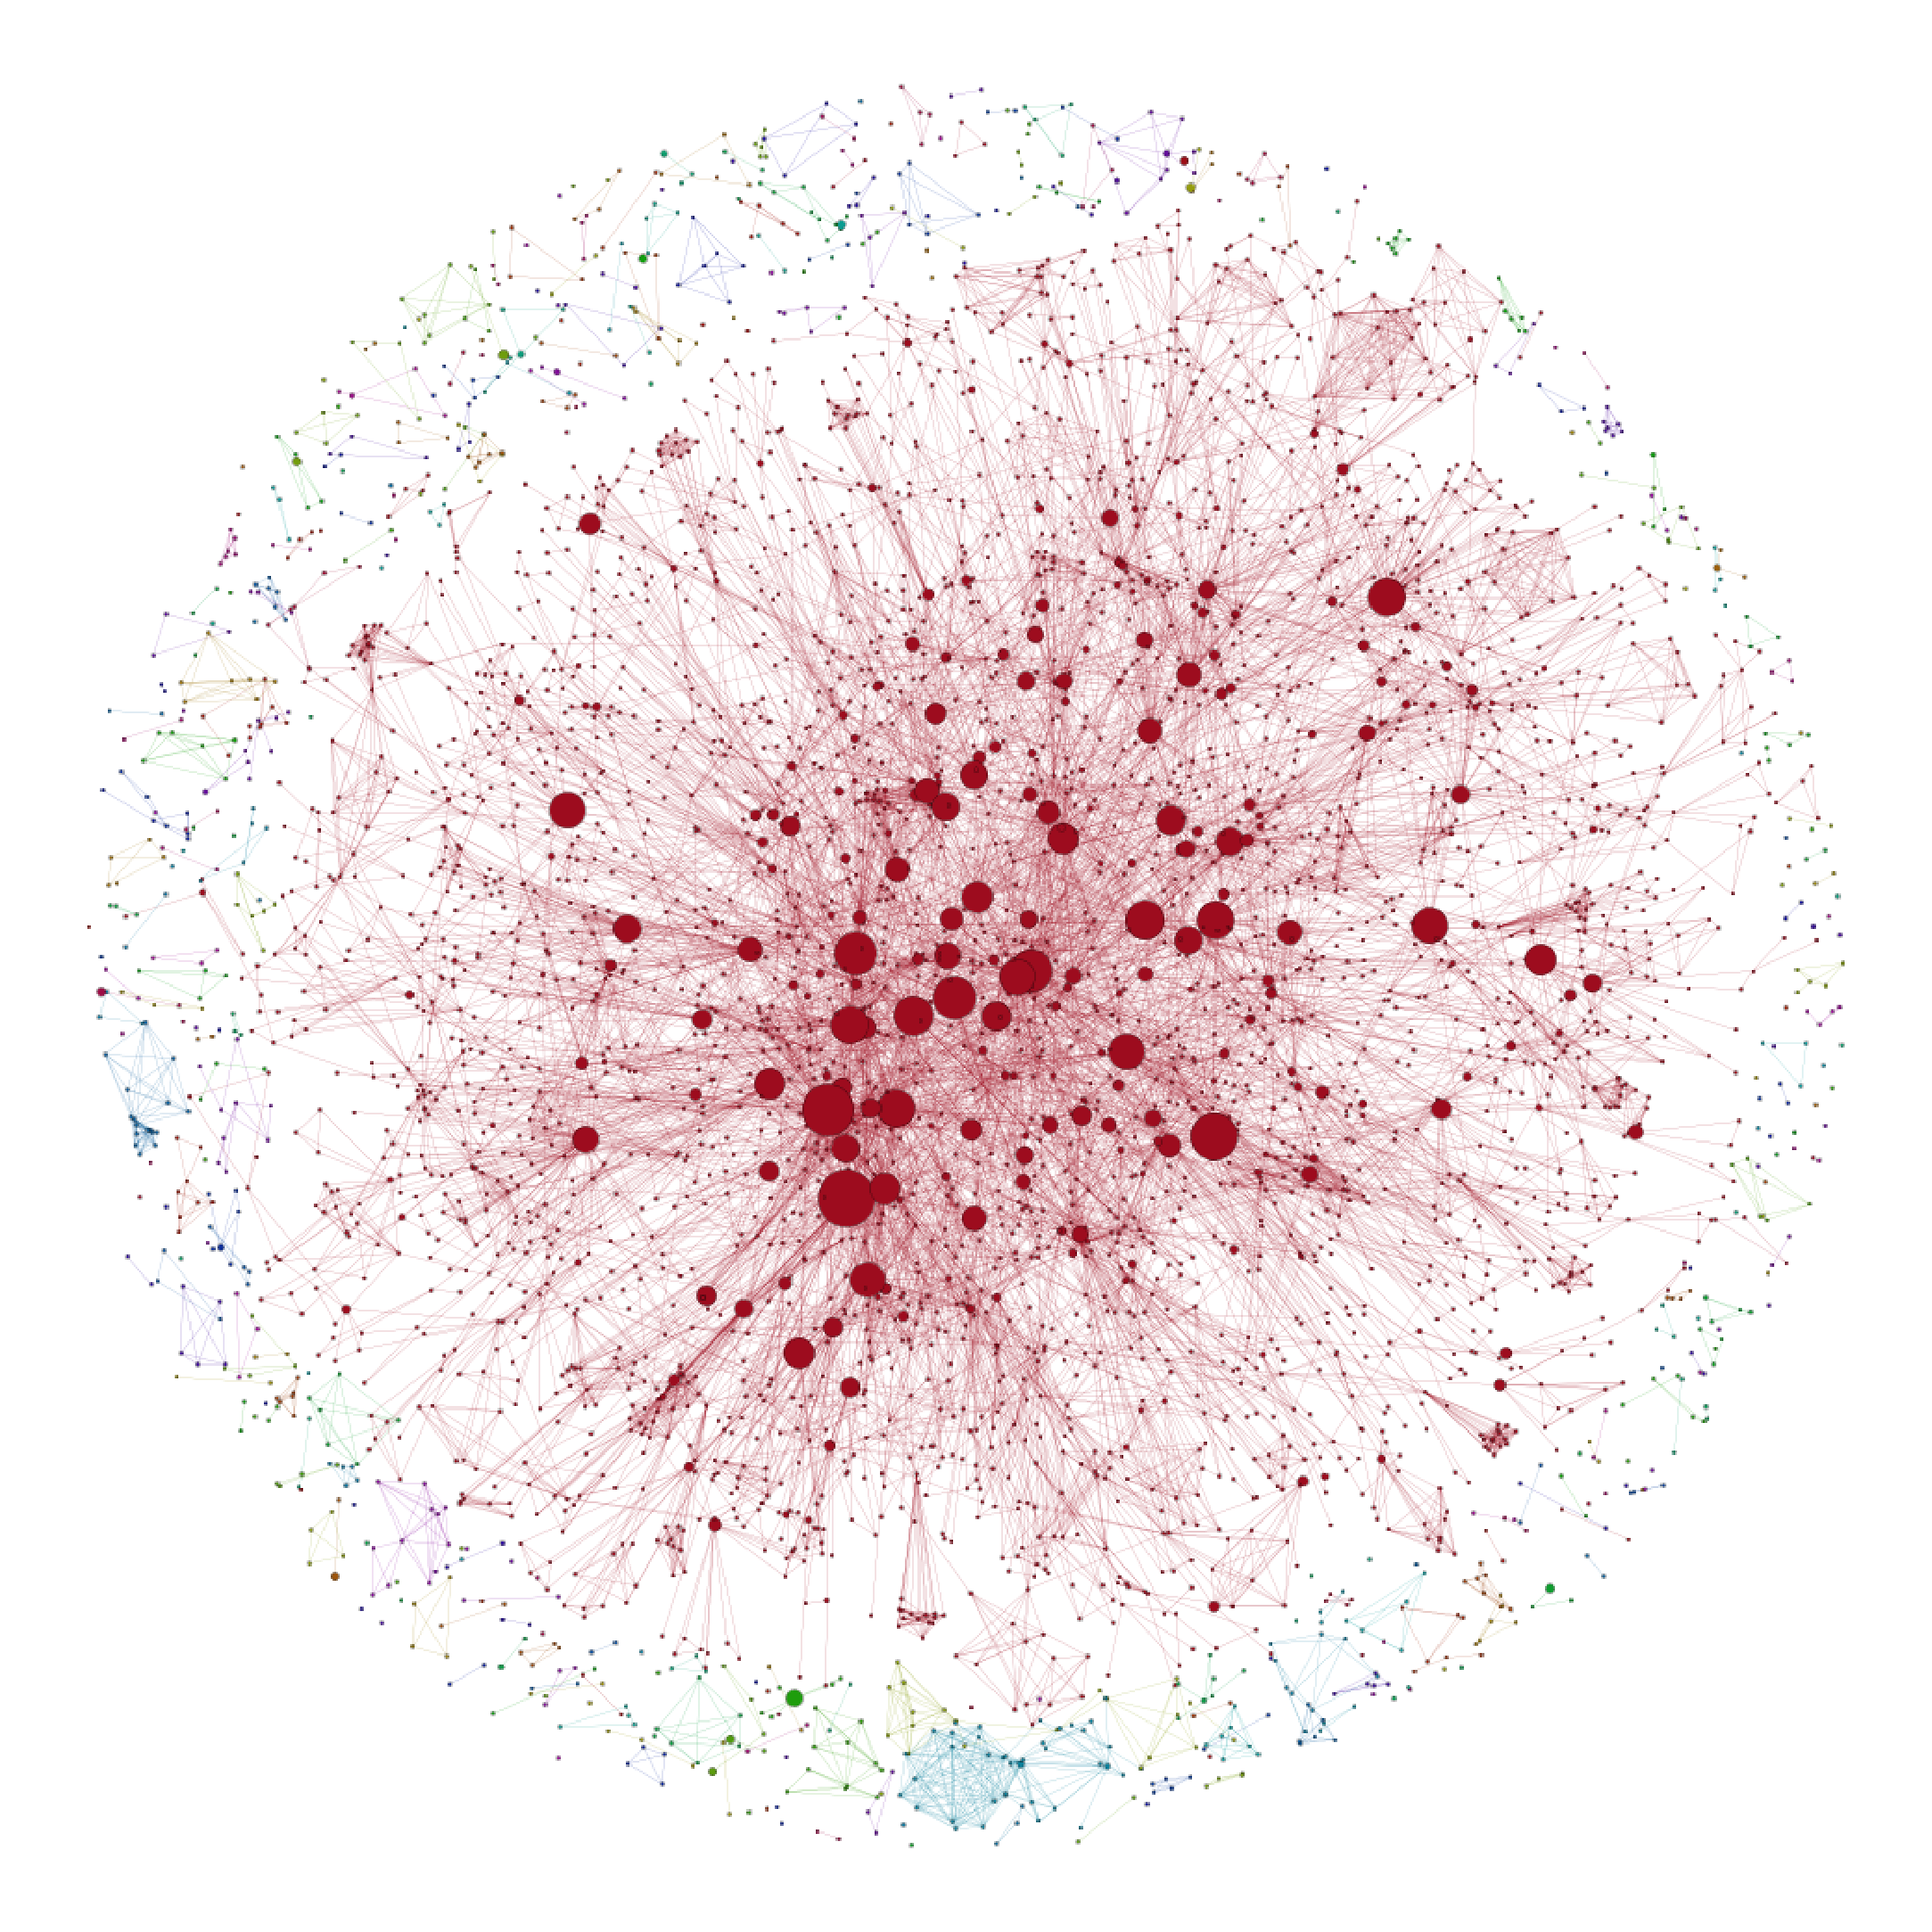
\includegraphics[scale=.16]{../graficos/network/sigmod.eps}
  }%
  \subfigure[CHI]{%
    \label{fig:rede_chi}
    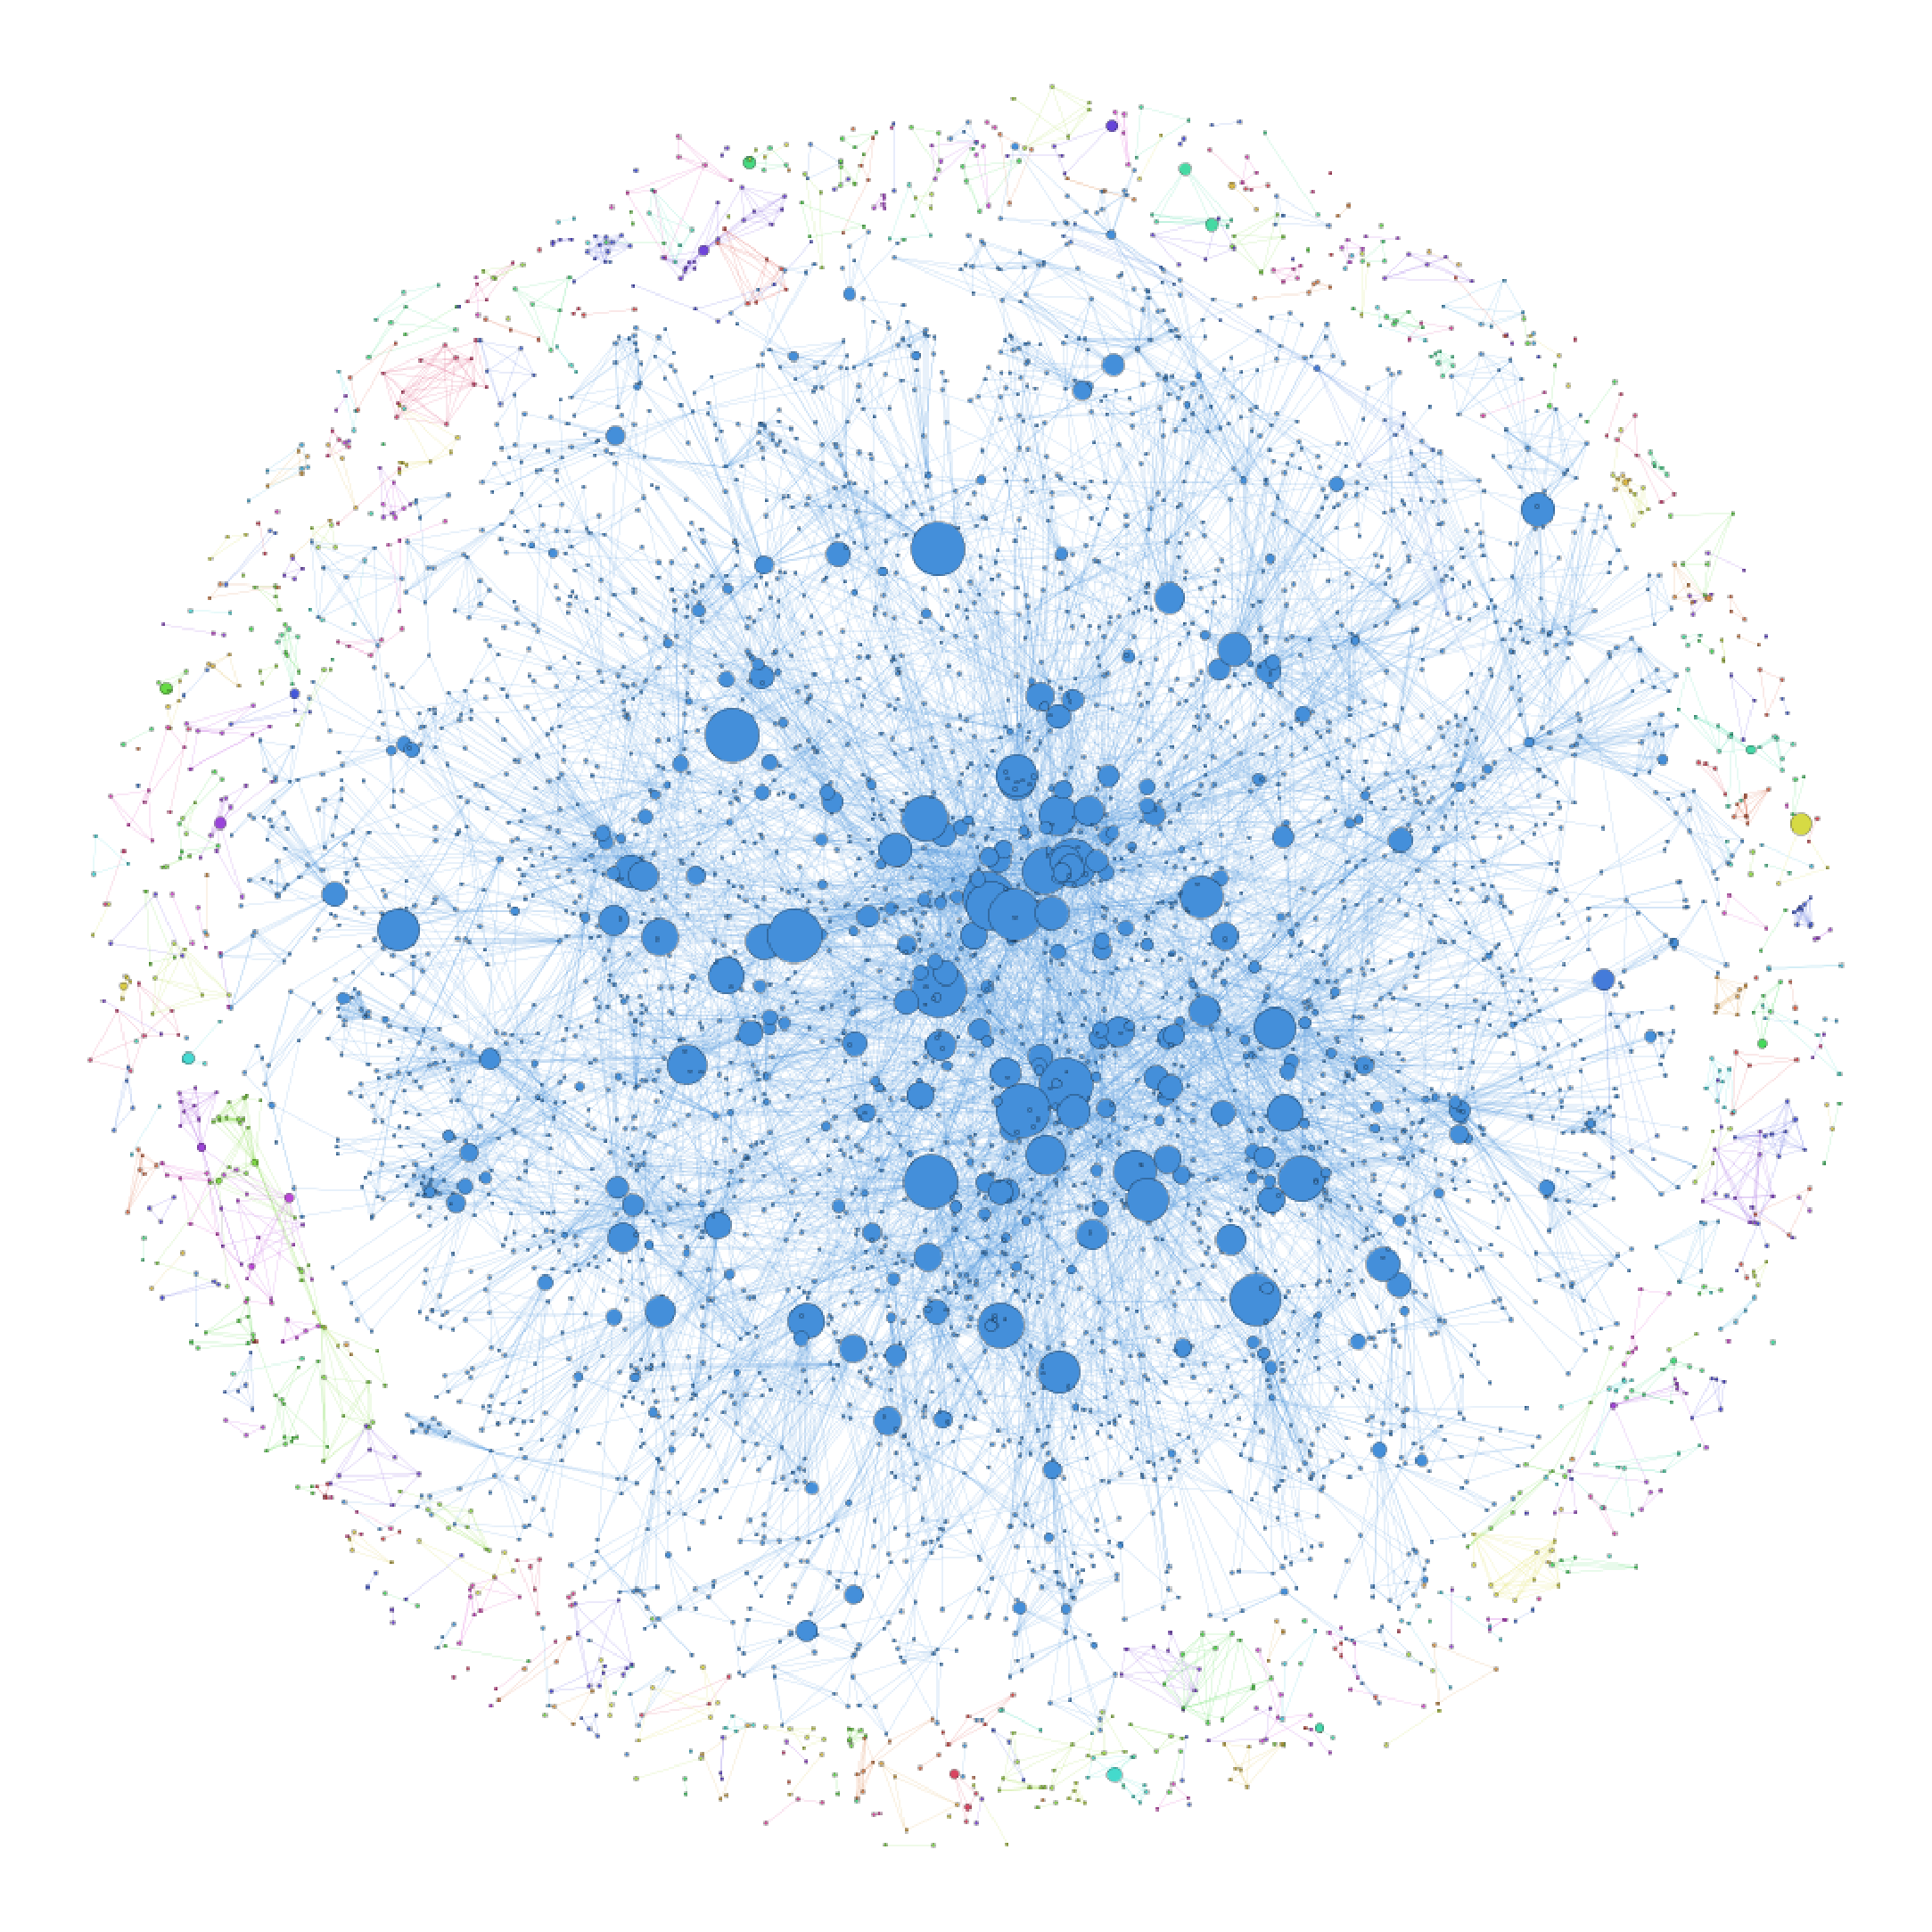
\includegraphics[scale=.16]{../graficos/network/chi.eps}
  }%
  \end{center}
  \caption{Instância final das comunidades científicas}
  \label{fig:redes}
\end{figure}

A partir dos resultados do nosso estudo, identificamos algumas oportunidades 
de trabalhos futuros, por exemplo, aplicação da métrica \textit{CoScore} a 
outros contextos, utilização de outras métricas de prolificidade, geração de 
modelos de formação de comunidades, aplicação da abordagem proposta 
para o estudo de \textit{clusters} e análise do impacto da migração de 
pesquisadores entre comunidades.

\bibliographystyle{sbc}
\bibliography{resumo-csbc}

\end{document}
